\begin{figure}[htbp]
	% Partly taken from http://www.texample.net/tikz/examples/convolution-of-two-functions/
	\centering
	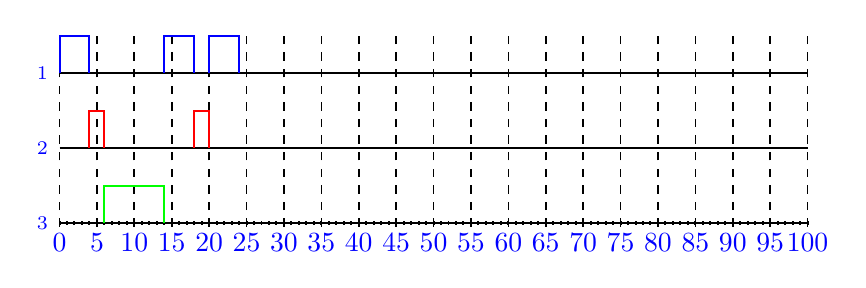
\begin{tikzpicture}[
		scale=0.095,
		line width=0.25mm,
		every node/.style={scale=1, text=blue},
		major tick/.style={semithick, dashed},
		x tick label/.style={anchor=north, minimum width=5mm},
		task1/.style={blue},
		task2/.style={red},
		task3/.style={green},
		desc/.style={anchor=east}
		]		

	% Task 1
	\draw (0, 20) -- (100, 20);
	\node[desc] at (0, 20) {$\uptau_1$};		
	
	% Task 2
	\draw (0, 10) -- (100, 10);
	\node[desc] at (0, 10) {$\uptau_2$};	
	
	% Task 3
	\draw (0, 0) -- (100, 0);
	\node[desc] at (0, 0) {$\uptau_3$};	
	
	% Small ticks
	\foreach \x in {0, 1,...,100}{
		\draw (\x, -0.25) -- (\x, 0.25);
	}
	
	% Major ticks with label
	\foreach \x/\label in {0, 5,...,100}{
		\node[x tick label] at (\x, 0) {$\label$}; 		
		\draw[major tick] (\x, -0.5) -- (\x, 26);
	}

	\draw[task1] (0, 20) -- (0, 25) -- (4, 25) -- (4, 20);
	\draw[task2] (4, 10) -- (4, 15) -- (6, 15) -- (6, 10);
	\draw[task3] (6, 0) -- (6, 5) -- (10, 5); % Wait, EDF!
	\draw[task3] (10, 5) -- (14, 5) -- (14, 0); % ok, go on!
	\draw[task1] (14, 20) -- (14, 25) -- (16, 25);
	\draw[task1] (16, 25) -- (18, 25) -- (18, 20);
	\draw[task2] (18, 10) -- (18, 15) -- (20, 15) -- (20, 10);
	\draw[task1] (20, 20) -- (20, 25) -- (24, 25) -- (24, 20);
%	\draw[task3] (24, 0) -- (24, 5) -- (30, 5); % ok, go on!
%	\draw[task3] (30, 5) -- (32, 5) -- (32, 0); % ok, go on!
%	\draw[task1] (32, 20) -- (32, 25) -- (36, 25) -- (36, 20);
%	\draw[task2] (36, 10) -- (36, 15) -- (38, 15) -- (38, 10);
%	\draw[task1] (40, 20) -- (40, 25) -- (44, 25) -- (44, 20);
%	\draw[task3] (44, 0) -- (44, 5) -- (48, 5); % ok, go on!
%	\draw[task3] (48, 5) -- (50, 5); % ok, go on!
%	\draw[task3] (50, 5) -- (52, 5) -- (52, 0); % ok, go on!
%	\draw[task1] (52, 20) -- (52, 25) -- (56, 25) -- (56, 20);
%	\draw[task2] (56, 10) -- (56, 15) -- (58, 15) -- (58, 10);
%	\draw[task1] (60, 20) -- (60, 25) -- (64, 25) -- (64, 20);
%	\draw[task2] (64, 10) -- (64, 15) -- (66, 15) -- (66, 10);
%	\draw[task3] (66, 0) -- (66, 5) -- (70, 5); % ok, go on!
%	\draw[task3] (70, 5) -- (74, 5) -- (74, 0);
%	\draw[task1] (74, 20) -- (74, 25) -- (78, 25) -- (78, 20);
%	\draw[task1] (80, 20) -- (80, 25) -- (84, 25) -- (84, 20);
%	\draw[task2] (84, 10) -- (84, 15) -- (86, 15) -- (86, 10);
%	\draw[task3] (86, 0) -- (86, 5) -- (90, 5); % ok, go on!	
%	\draw[task3] (90, 5) -- (94, 5) -- (94, 0);
%	\draw[task1] (94, 20) -- (94, 25) -- (96, 25);% ok, go on!
%	\draw[task1] (96, 25) -- (98, 25) -- (98, 20);	
%	\draw[task2] (98, 10) -- (98, 15) -- (100, 15) -- (100, 10);

	\end{tikzpicture}
%	\caption{Ablaufübersicht}
\end{figure} 